% ---------
%  Compile with "pdflatex hw0".
% --------
%!TEX TS-program = pdflatex
%!TEX encoding = UTF-8 Unicode

\documentclass[11pt]{article}
\usepackage{jeffe,handout,graphicx,mathtools}
\usepackage[utf8]{inputenc}		% Allow some non-ASCII Unicode in source
\usepackage{enumerate}
\usepackage{fourier-orns}
\usepackage{tikz}
\usetikzlibrary{automata, positioning}

%  Redefine suits
\usepackage{pifont}
\def\Spade{\text{\ding{171}}}
\def\Heart{\text{\textcolor{Red}{\ding{170}}}}
\def\Diamond{\text{\textcolor{Red}{\ding{169}}}}
\def\Club{\text{\ding{168}}}

\def\Cdot{\mathbin{\text{\normalfont \textbullet}}}
\def\Sym#1{\textbf{\texttt{\color{BrickRed}#1}}}

\newcommand{\comp}[1]{#1_{\text{comp}}}
\input{macros}
\newtheorem{lemma}{Lemma}


% =====================================================
%   Define common stuff for solution headers
% =====================================================
\Class{CS/ECE 374}
\Semester{Spring 2017}
\Authors{2}
\AuthorOne{Renheng Ruan}{rruan2}
\AuthorTwo{Lanxiao Bai}{lbai5}

%\Section{}

% =====================================================
\begin{document}

% ---------------------------------------------------------


\HomeworkHeader{2}{3}	% homework number, problem number

\begin{quote}
\begin{enumerate}[(a)]
\item Describe a concrete example of a machine $N$
 to show that $L(\comp{N}) \neq \overline{L(N)}$. You need
 to explain for your machine $N$ what $\overline{L(N)}$ and
 $L(\comp{N})$ are.

\item
Define an NFA that accepts 
$\overline{L(N)} - L(\comp{N})$, and explain how it works.

\item
Define an NFA that accepts 
$L(\comp{N}) - \overline{L(N)}$, and explain how it works.

\end{enumerate}
\end{quote}
\hrule

\begin{solution}
	\mbox{}
\begin{enumerate}[(a)]
\item
\mbox{}
\begin{figure}[h]
	\begin{center}
		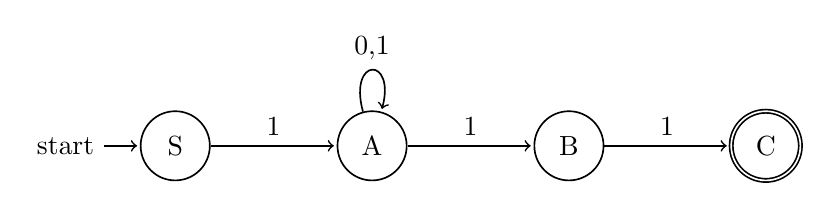
\begin{tikzpicture}[shorten >=1pt, auto, node distance=2.5cm, 
		semithick]
		\node[state, initial] (S) {S};
		\node[state] (A) [right of=S] {A};
		\node[state] (B) [right of=A] {B};
		\node[accepting,state] (C) [right of=B] {C};
		
		\path[->]
		(S) edge node {1} (A)
		(A) edge [loop above] node {0,1} (A)
		(A) edge node {1} (B)
		(B) edge node {1} (C);
		\end{tikzpicture}
	\end{center}
	\caption{}
\end{figure}
\begin{figure}[h]
	\begin{center}
		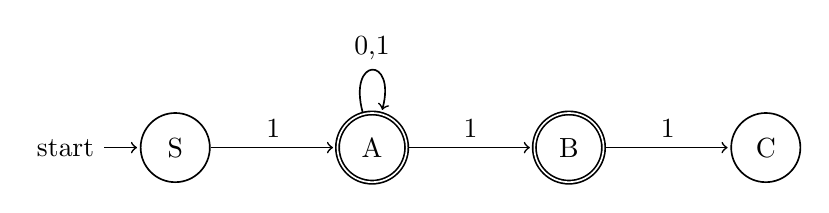
\begin{tikzpicture}[shorten >=1pt, auto, node distance=2.5cm, 
		semithick]
		\node[initial,state] (S) {S};
		\node[accepting,state] (A) [right of=S] {A};
		\node[accepting,state] (B) [right of=A] {B};
		\node[state] (C) [right of=B] {C};
		
		\path[->] 
		(S) edge node {1} (A)
		(A) edge [loop above] node {0,1} (A)
		(A) edge node {1} (B)
		(B) edge node {1} (C);
		\end{tikzpicture}
	\end{center}
	\caption{}
\end{figure}

Let $L({N}) = L(1(0 + 1)^{*}11)$, as in figure 1, then $\overline{L(N)}$ does not end with $11$. By swapping the accept and non-accept states which is shows as figure 2, $L(\comp{N})$ accepts $011$, however, $\overline{L(N)}$ does not end with $11$, so that $L(\comp{N}) \neq \overline{L(N)}$.$\blacksquare$


\begin{lemma}
	Let $A, B \subseteq Q$ and $\delta(S, w_1) = \{A, B\}, \delta(S, w_2) = \{A\}, \delta(S, w_3) = \{B\},\delta(S, w_4) = \emptyset$. If N accepts both $w_1$ and $w_2$,
then $N'$ that accepts $\overline{L(N)}$ accepts both $w_3$ and $w_4$,
and $\comp{N}$ accepts both $w_1$ and $w_3$. Denote $L_1 = \{w : \delta(S, w) = \{A, B\}\}, L_2 = \{w : \delta(S, w) = \{A\}\}, L_3 = \{w : \delta(S, w) = \{B\}\}, L_4 = \{w : \delta(S, w) = \emptyset \}$.
\end{lemma}

\paragraph{Proof:} This lemma is true by the definition of NFA.$\blacksquare$

\item
By Lemma 1,
\begin{center}
	$\overline{L(N)} - L(\comp{N}) = L_3 + L_4 - (L_1 + L_3) = L_4 = \emptyset$
\end{center}

\item  
By Lemma 1,
\begin{center}
	$L(\comp{N}) - \overline{L(N)}$ = $L_1 + L_3 -(L_3 + L_4)$ = $L_1$ = $A + B$
\end{center}

\end{enumerate}
\end{solution}

\end{document}
